\documentclass[usenames, dvipsnames, twocolumn]{article}
\usepackage[utf8]{inputenc}


\newcommand{\mytitle}{A Hybrid Physical \& Statistical Approach to Storm Surges}
\newcommand{\penname}{Candidate 8205R}
\newcommand{\supervisor}{\\Supervisor:\\  Dr. Dan Jones,\\ British Antarctic Survey}


\usepackage{Theme/mystyle}
\usepackage{Theme/globals}
% Define some vital globals for the document etc.

% Where I put the images to be imported.
\graphicspath{{images/}{../images/}}

\addbibresource{references/generic_references.bib}
\addbibresource{references/references.bib}
\addbibresource{references/fluid_dynamics.bib}
\addbibresource{references/machine_learning.bib}
\addbibresource{references/global_warming.bib}
\addbibresource{references/programming.bib}
\addbibresource{references/surge.bib}
\addbibresource{references/tebbutt.bib}
\addbibresource{references/taleb.bib}
\addbibresource{references/evt.bib}
\addbibresource{references/cyclone.bib}
\addbibresource{references/meteorology.bib}
  % bibliography added here

\usepackage{cleveref}
% I prefer the automatic § symbol when I'm referencing sections.
\crefformat{section}{§#2#1#3}
\crefformat{subsection}{§#2#1#3}
\crefformat{subsubsection}{§#2#1#3}

\setlength\headheight{26pt} %% just to make a warning go away.
\rhead{\thepage}  % right head page number.
% page number on right head
\lfoot{\penname}  % left foot author.
\cfoot{}
\rfoot{}
\pagestyle{fancy}  % use fancyhdr style

\date{January 2020}
\title{\vspace*{-100pt}\textbf{\mytitle}\vspace{-10pt}}
\author{\penname \\  \supervisor }
\immediate\write18{texcount -nc -inc -merge -sum -q proposal.tex > wordcount/prop_wordcount.tex}


\begin{document}
  \begin{@twocolumnfalse}
    \vspace{-25pt}
  \maketitle
  \setcounter{page}{1}
    \textsc{Initial Report submitted for Standard Credit in
the Natural Sciences Tripos}
    \begin{abstract}
     I set out a proposal for research which will be completed over the 8 weeks of Lent term.
     In an attempt to minimise research risk, there is significant flexibility on which data sources to focus on,
      and which theoretical frameworks to follow.
      The motivation for studying storm surges is described and they are put in their physical context.
      The project can be categorized as machine learning (ML) enabled climate physics,
       and will involve a significant amount of physical and algorithmic theory.
       See Figure~\ref{fig:Plan} for a project timeline.

\paragraph{Keywords:} \textit{Gaussian Processes, Climate Change,
 Non-Linear Physics, Fluid Mechanics.}
    \vspace{20pt}
    \end{abstract}

  \end{@twocolumnfalse}
\vspace{-30pt}
\noindent
\begin{figure}[htb!]
    \centering
    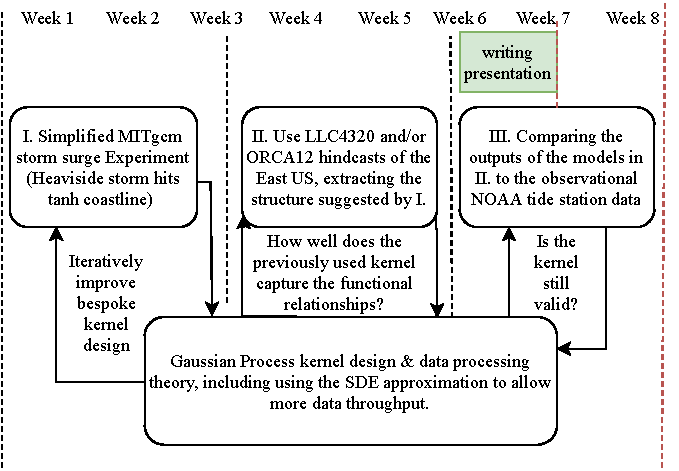
\includegraphics[width=\linewidth]{images/proposal/PartIIIProjPlan.pdf}
    \caption{A rough timeline of tasks for the project.}
    \label{fig:Plan}
\end{figure}

\vspace{-20pt}
\begin{quote}
    ``the true logic for this world is the calculus of Probabilities,
     which takes account of the magnitude of the probability which is,
      or ought to be, in a reasonable man’s mind.''
— James Clerk Maxwell [1850]~\cite{williams2006gaussian}
\end{quote}


\section{Supervision}

I will be primarily supervised by Dr.\ Dan Jones,
and have been granted visiting scientist status at the
British Antarctic Survey (BAS).
 Dr.\ Laure Zanna\footnote{Formerly of the Oxford Department of Physics.},
  New York University,
has also agreed to be an unofficial co-supervisor, as
she is interested in this area of work~\cite{ZannaPreprint, wilson2013tide,
 bolton2019applications}.
 I am a member of the BAS Artificial Intelligence lab, and so may
have the opportunity to ask Dr.\ Anita Faul\footnote{Formerly of the Cavendish Scientific-Computing Lab.}~\cite{faul2019concise}
 and Dr.\ J.\ Scott Hosking~\cite{bruinsma2019scalable}
technical questions.

I will present my preliminary results to the AI4ER-CESDG meeting on the Thursday of week 8.
This group provides an invaluable source of technical knowledge, as this Michaelmas we have
already had talks using Gaussian Processes for statistical downscaling
(Risa Ueno), aerosol model emulation (Dr.\ Lindsey Lee),  to predict
rain-driven flooding (Robert Rouse), and to combine GCMs (William Tebbutt).

\section{Motivation}


The timing of this project is quite auspicious, as it comes just after the publication
 of the IPCC's Special Report on the Oceans and Crysosphere in a Changing Climate (SROCC)~\cite{SROCC}.
  One of the headline results of this report was that in the most severe climate change scenario (RCP8.5),
   due to sea level rise alone, the current once in a century storm surge event would become a once per year event globally.
    The University has also just launched Cambridge Zero, and the Artificial Intelligence for Environmental Risk (AI4ER) CDT,
     both led by Dr.\ Emily Shuckburgh.

As a city near the East Coast of England, the risk of
storm surges is particularly relevant to Cambridge;
it is one of the few natural disasters that
poses a major risk to the United Kingdom, particularly in the nearby cities of
Lincoln and London. This project will focus on the East coast of the United States because it is
 (a) more densely instrumented, (b) at higher risk, and
 (c) better studied in the published literature~\cite{ZannaPreprint},
 so the novel methods tried here can be better compared against traditional methods.
  Future work could involve applying the same statistical modelling to the East Coast of England,
   as in  Wilson~et~al.~2013~\cite{wilson2013tide}.

Storm surges are difficult to model because they are (i) infrequent, (ii) short in time and space,
and  (iii) cannot be modelled well using linear analytic approximations.
Therefore, to deal with them easily using classical
frequentist statistics you would need a large amount of high spatial and temporal resolution
model data, from an unbiased model that matched the patterns of observations well in
its hindcasts. Sadly, such a model (or ensemble of models) is currently too
computationally expensive to run.  We must make do with more limited resources
 (listed in the following section), which justifies using the Bayesian non-parametric
  method of Gaussian Processes to get more from imperfect data, whilst retaining
   knowledge of the associated uncertainty.

Society has no reason to decide to change policy if the costs of the changes are greater than the risks that they avert. As scientists, we have to avoid the Scylla of overstating our findings, and the Charybdis of not providing the public with an adequate estimate of the potential risk associated with each course of action.

\section{Data Resources}

\begin{table}[htb!]
    \centering
    \begin{tabular}{rlr}
                 & \textbf{Resource} & \textbf{Location} \\
        \textbf{A} & MITgcm Experiment~\cite{marshall1998efficient, marotzke1999construction}\footnotemark & BAS HPC \\
        \textbf{B} & LLC4320~\cite{Abernathey2017} & Pangeo Catalog\\
        \textbf{C} & ORCA12~\cite{treguier2017orca12} & JASMIN HPC \\
        \textbf{D} & NOAA Tidal Gauges & Online API  \\
    \end{tabular}
    \caption{The relevant datasets available.}
    \label{tab:data_sources}
\end{table}
\footnotetext{\url{https://mitgcm.readthedocs.io/en/latest/examples/plume_on_slope/plume_on_slope.html}}
See Table~\ref{tab:data_sources} for a the list of relevant data sources I have
 located.\footnote{Tidal gauge data (including meteorological) available at
  \url{https://tidesandcurrents.noaa.gov/api-helper/url-generator.html}}
   Figure~\ref{fig:tile10} shows some data from LLC4320 which can be easily
    accessed and plotted. LLC4320 is a 2km resolution model produced with MITgcm
     with time steps every hour for the year Sept-2011 to Sept-2012.

ORCA12 is also a \(\frac{1}{12}^{\circ}\) coupled climate model,
 and we have managed to secure hourly outputs for the year 2005 from the MET Office,
  although these have not yet been transferred to the JASMIN HPC.

\begin{figure}[htb!]
    \centering
    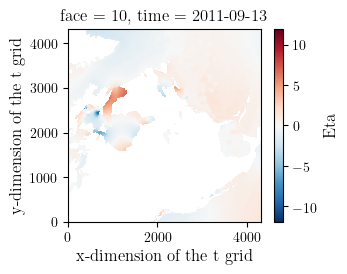
\includegraphics[width=0.8\linewidth]{images/proposal/tile10.png}\\
    \caption{An unfortunately orientated plot of sea surface height,
     for the 10th face of LLC4320.}
    \label{fig:tile10}
\end{figure}

\begin{figure}[htb!]
    \centering
    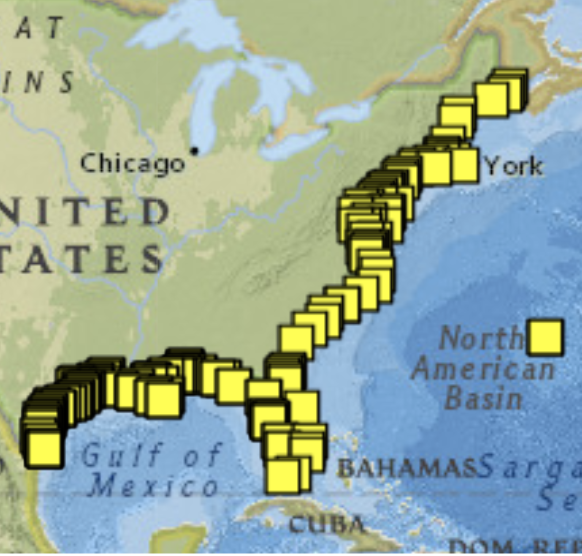
\includegraphics[width=0.8\linewidth]{images/proposal/TidalGaugesUS.png}\\
    \textit{Figure Source: \url{https://www.ngdc.noaa.gov/hazard/tide/#}}
    \caption{A map showing NOAA tidal gauges placed on the East Coast.}
    \label{fig:tidal}
\end{figure}
\section{Physical Problem}


How will the frequency and intensity of storm surge events change over time
 in the North-Eastern United States as global temperatures increase?
  This question is easily stated, but difficult to properly answer.

The earth’s climate system is dominated be the action of 3 fluids: the ice,
 atmosphere, and oceans. The equations that govern these are simple if non-linear.
  A fundamental problem with the attempts to model the interaction between these
   three fluids is that the Earth is large, and so the resolution that can be
    achieved in reasonable computational time is much larger than a fluid element
      (\(\frac{1}{12}^{\circ}\) or \(\sim\)8km in the most recent round of global
       coupled models\footnote{i.e.\ CMIP6}). Therefore, to capture the behaviours
        that happen sub-grid scale these must be parameterised back into the model.~\cite{powell2003reduced}

These parameterisations allow global coupled models (GCMs) to be reasonable guides to mean global and regional properties, but are shown to be systematically biased in their distribution at a specific location when GCM runs of the past are compared against observational data. This bias can be assumed to be approximately the same if that weather state reoccurs; if we know how much the model was off by in a specific weather state in the past, and if the same weather state occurs in the future, then the same transformation will be valid to produce a corrected version of the future climate.

By analogy, this is similar to the assumption that the states of the new climate are approximately the same as the old climate, but the distribution among those states has changed. This still begs the question of what can be assumed to be the same weather state, as these states are not discrete, and no two weather states are truly identical.

The first part of the project will focus on understanding
whether the weather state can be well labelled by proximal
indicators at a location, and how relevant each indicator is.

Many different simplifications can be made to the full equations of fluid motion, such as the shallow water equations.
The shallow water equations are:
    \begin{eqnarray}
    \frac{Du}{Dt} + \underline{f}\times\underline{u} = - g \underline{\nabla} \eta \; \\
\frac{Dh}{Dt} + h \underline{\nabla}\cdot\underline{u} = 0  \Leftrightarrow \frac{\partial h}{\partial t} + \underline{\nabla}\cdot(h\underline{u})= 0 \\
w. \quad \quad h(x, y , t) = \eta(x, y, t) - \eta_{b}(x, y)\\
\& \quad \frac{D}{Dt}= \frac{\partial}{\partial t} + \underline{u}\cdot\underline{\nabla} = \dfrac{\partial}{\partial t} + u \frac{\partial}{\partial x} + v \dfrac{\partial}{\partial y}
    \end{eqnarray}

\section{Gaussian Processes (GPs)}
\afterpage{
\begin{figure*}[p]

    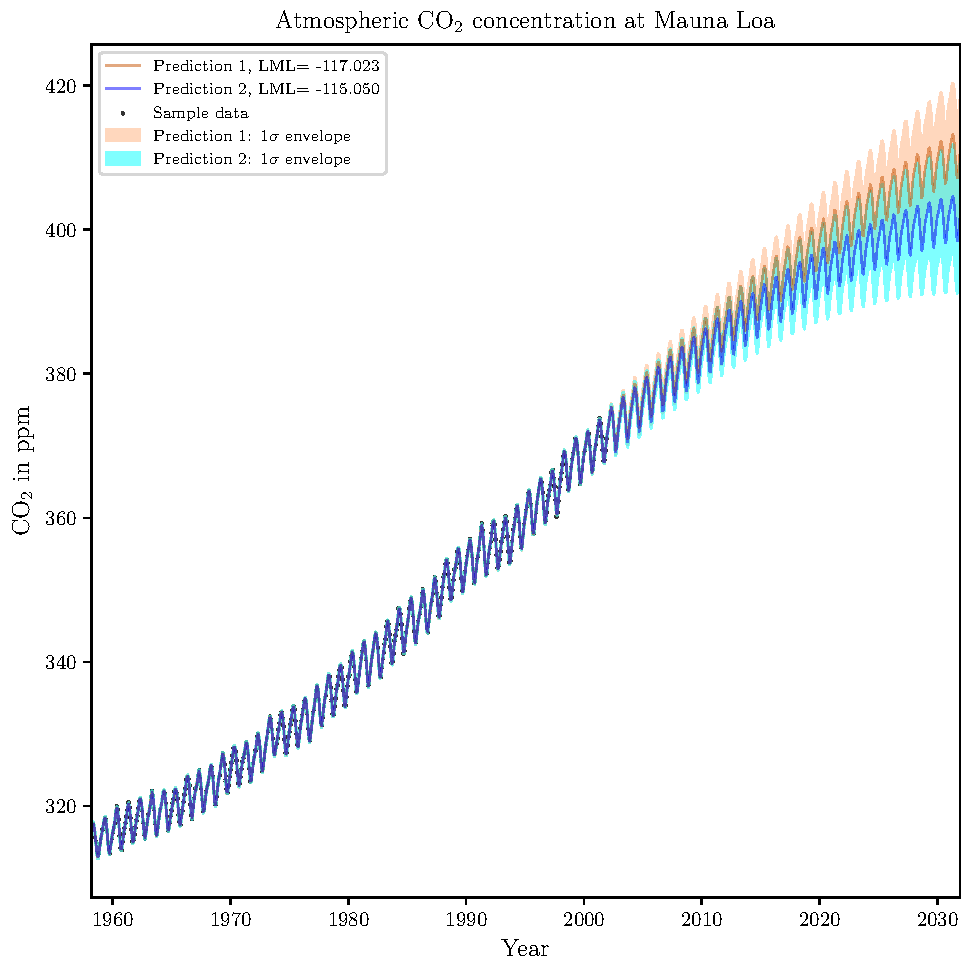
\includegraphics[width=\linewidth]{images/proposal/mauna-loa_gpr_co2_combined.pdf}

    \vspace{-10pt}

    \caption{
        An example of Gaussian Process regression (Kriging) to the observational data from the station at Mauna Loa.
        A local maximum in Log-Marginal Likelihood is found, which is dependent on the initial conditions of the kernel, but with no guarantee of this being global. In this case we should prefer Prediction 2 to Prediction 1 because it has a higher LML (see Table~\ref{tab:GP_CO2}), which would suggest that the case with substantially lower CO$_2$ concentration by 2030 is more likely given the data. However this is weak inference because: (a) the Kernel we have used does not encode all of our prior knowledge about the system and has no non-stationary components (b) I cannot guarantee that this is the global maximum in Log-Marginal Likelihood (c) the GP has been trained on a limited dataset from the last half century, and the trend that it picks out could be sensitive to the start date (d) given only 50 years of data the larger period components of the signal will be subject to aliasing.
        }
        \label{fig:GP_CO2}
\end{figure*}
}

\subsection{Theoretical Justification}


Gaussian Processes (GPs) are a popular tool within probabilistic machine learning (ML), and the field predominantly uses Williams and Rasmussen's textbook~\cite{williams2006gaussian}\footnote{\href{http://www.gaussianprocess.org/gpml/chapters/RW.pdf}{http://www.gaussianprocess.org/gpml/chapters/RW.pdf}},
Researchers prize GPs' ability to produce a data-driven prediction of a value with an associated uncertainty distribution given some number of inputs~\cite{ebden2008gaussian}.\footnote{ \href{https://www.robots.ox.ac.uk/~mebden/reports/GPtutorial.pdf}{https://www.robots.ox.ac.uk/$\sim$mebden/reports/GPtutorial.pdf}}. The GP is completely described by its mean prediction value \(m(\mathbf{x})\) and its covariance \(k\left(\mathbf{x}, \mathbf{x}^{\prime}\right)\) through
\begin{equation}m(\mathbf{x})=\mathbb{E}[f(\mathbf{x})], \end{equation}\begin{equation}k\left(\mathbf{x}, \mathbf{x}^{\prime}\right)=\mathbb{E}\left[(f(\mathbf{x})-m(\mathbf{x}))\left(f\left(\mathbf{x}^{\prime}\right)-m\left(\mathbf{x}^{\prime}\right)\right)\right].\end{equation}
With the GP written as:
\begin{equation}f(\mathbf{x}) \sim \mathcal{G} P\left(m(\mathbf{x}), k\left(\mathbf{x}, \mathbf{x}^{\prime}\right)\right). \end{equation}

The field of fluid dynamics is considering the ways to use
Machine Learning to interpret data~\cite{brenner2019perspective},
and non-Bayesian techniques such as deep learning
have been successfully to predict things such as arctic sea
ice~\cite{ham2019deep, bolton2019applications}.
I choose not to use these methods because while they `work
well', they are very hard to interpret, and so their ability to
add scientific knowledge is impaired. The uncertainty in their
predictions is often unclear, so that in unseen climate states
they might predict a certain event with spurious certainty.

\subsection{Choosing a Kernel}
Writing a bespoke kernel to solve your optimisation problem is advised~\cite{duvenaud2014automatic},
as you should be the expert in the modelling problem that you are trying to
solve rather than using something generic~\cite{LeMaitre2019gaussian,
 duvenaud2014automatic}\footnote{\href{https://www.cs.toronto.edu/~duvenaud/cookbook/
}{https://www.cs.toronto.edu/$\sim$duvenaud/cookbook/}}.

It is common to interpret the GP kernel,
and its initial state as a prior expectation
about what you expect the functional form of the relationship between different
variables to be.

However it is quite common to start from common, pre-written kernels,
as the process of deciding on a kernel is complicated. The late Professor Sir David
Mackay~\cite{ITILA}\footnote{(see Durrande 2016 ~\cite{durrande2016detecting} for attribution)} first derived the periodic kernel (also known as \texttt{ExpSineSquared}),
\begin{equation} k_{\mathrm{periodic}}\left(x_{i}, x_{j}\right) =\nu^{2}
 \exp \left(-\frac{2 \sin ^{2}\left(\frac{\pi}{T}\left|x_{i}-x_{j}\right|\right)}{\lambda_{1}^{2}} \right), \end{equation}
which can be used to fit data with a particular periodicity. Another popular kernel is the radial basis function kernel (\texttt{RBF}),
\begin{equation} k_{\mathrm{RBF}}\left(x_{i}, x_{j}\right)=\nu^{2} \exp \left(-\frac{\left|x_{i}-x_{j}\right|^{2}}{2 \lambda^{2}}\right), \end{equation}
which encodes a smoothness with a particular length scale to the form of the function.

I will be using the package Sci-Kit-Learn (\texttt{sklearn}) from within Python3, which has a number of kernels (\texttt{RBF}, \texttt{ExpSineSquared}, \texttt{DotProduct}, \texttt{ConstantKernel}, \texttt{RationalQuadratic}, \texttt{WhiteKernel},  and \texttt{Matern}) built-in, and these can be combined together using \texttt{Sum}, \texttt{Product}, or \texttt{Exponentiation} which allows significant flexibility to the final form of the kernel, enough that a relatively common strategy is to iteratively guess
a kernel until the Gaussian Process fits the data well.\footnote{The automated statistician project attempts to solve this problem \url{https://automaticstatistician.com/about/}}

 Figure \ref{fig:GP_CO2}\footnote{
    This example was originally taken from
    \href{https://scikit-learn.org/stable/modules/gaussian_process.html}{https://scikit-learn.org/stable/modules/gaussian\_process.html}.}
shows using Gaussian Processes to fit observational CO$_2$ data using a
combination of \texttt{RBF}, \texttt{ExpSineSquared}, \texttt{RationalQuadratic}
 and \texttt{WhiteKernel},
as shown in Table~\ref{tab:GP_CO2}.

 \begin{table}
\begin{tabular}{p{0.49\textwidth}}
        \textbf{Prediction 1 (LML=-117):}\\
        \texttt{66**2 * RBF(length\_scale=67)}\\
        \texttt{+ 2.4**2 * RBF(length\_scale=90)}\\
        \texttt{* ExpSineSquared(length\_scale=1.3, periodicity=1)}\\
        \texttt{+ 0.66**2 * RationalQuadratic(alpha=0.78, length\_scale=1.2)}\\
        \texttt{+ 0.18**2 * RBF(length\_scale=0.134)}\\
        \texttt{+ WhiteKernel(noise\_level=0.0361)}\\
        \textbf{Prediction 2 (LML=-115):} \\
        \texttt{44.8**2 * RBF(length\_scale=51.6)}\\
        \texttt{+ 2.64**2 * RBF(length\_scale=91.5)}\\
        \texttt{* ExpSineSquared(length\_scale=1.48, periodicity=1)} \\
        \texttt{+ 0.536**2 * RationalQuadratic(alpha=2.89, length\_scale=0.968)}\\
        \texttt{+ 0.188**2 * RBF(length\_scale=0.122)} \\
        \texttt{+ WhiteKernel(noise\_level=0.0367)}
     \end{tabular}
     \caption{This example of fitting CO\(_2\) observations with a kernel
     (shown in Figure~\ref{fig:GP_CO2}) was originally taken from
    \href{https://scikit-learn.org/stable/modules/gaussian_process.html}{https://scikit-learn.org/stable/modules/gaussian\_process.html}.}
    \label{tab:GP_CO2}
     \end{table}


\subsection{Implementation}

A critical problem with using GPs for ML is that their most naive
 implementation GP run-time scales with \(\mathcal{O}(n^3)\),
where \(n\) is the number of observational inputs taken,
 because of the matrix operations that occur during convergence.
Even with HPC resources, and the Moore's law growth of capacity,
 this puts many applications out of reach.
However, there are various methods of reducing this cost through
approximations such as Stochastic Differential Equations which can be created to
have the same behaviour as a specific kernel and run with \(\mathcal{O}(n)\) complexity,
 as detailed in  \cite{marshall2019exploring,sarkka2019applied,titsias2009variational,solin2016stochastic},
  and I will try to implement this
or other methods to increase the amount of training data.

As mentioned, I will be using \texttt{sklearn}~\cite{scikit-learn} for ML. I will be using \texttt{xarray}~\cite{hoyer2017xarray} for high dimensional climate datasets and  \texttt{numpy}~\cite{numpy} for fast
python data analysis.

%\cite{sacks1989design}
\subsection{Other Problems with Gaussian Processes}
\subsubsection{The assumption of a Gaussian Error}
GPs assume that there is a Gaussian error around each point,
 but this is often not the case in real variables.
However, it is often possible to transform to a space where this is the case, Krige there,
 and then transform back~\cite{snelson2004warped}.\footnote{\url{http://mlg.eng.cam.ac.uk/zoubin/papers/gpwarp.pdf}}.
Lewis Fry Richardson (1948) showed that the estimates of deaths during a war had
 symmetric error bars in logarithmic space~\cite{richardson1948variation}.
\subsubsection{The assumption of zero mean}
Most practitioners of Gaussian Processes choose to have \(m(\mathbf{x})=0\)~\cite{williams2006gaussian}.
This can cause certain issues, particularly if there is a change
in the function across the range, such as a Heaviside step function,
as such a GP with \(m(\mathbf{x})=0\) could not tend to different values
at different ends of the number line.
If necessary, it is possible to learn the mean,
 though this will significantly increase the computational expense.


\section{MITgcm Experiment}
If a problem seems to difficult to know where to start, it is often a good strategy
to try to simplify it to the greatest extent possible,
solve that problem, and then use that as a starting guess when trying
to solve the full problem. In this spirit I propose that the project
should start by applying a Heaviside storm of various strengths against
a cartoon-like $\tanh$ coastline, where a single 2D slice is simulated
in the interest of limiting run-time, so that more conditions can be
simulated.

The Massachusetts Institute of Technology general circulation model
MITgcm~\cite{marshall1998efficient, marotzke1999construction} is widely used
 in oceanography~\cite{verdy2017data}, and relatively easy to use.
We have chosen the introductory exercise of this project to be
looking at a highly simplified version of the situation,
where a 2 dimensional slice of the coastline has bathymetry, \(H(x) \),
\begin{equation}
H(x) = -H_o + (H_o - h_s) ( 1 + \tanh{\left(\frac{x-x_s}{L_s}\right)} ) / 2 .
\end{equation}
Where the parameters are given by:
\begin{eqnarray}
H_o & = & 500 \;\; \mbox{(m)} \\
h_s & = & 0 \;\; \mbox{(m)} \\
x_s & = & [\sim1500] + L_x/2 \;\; \mbox{(m)} \\
L_s & = & \frac{(H_o - h_s)}{2 s} \;\; \mbox{(m)} \\
s & = & [\sim0.15]\\
L_x & = & 6400 \;\; \mbox{(m)},
\end{eqnarray}
where the square brackets indicate that the parameters will be varied. \(s\) is the maximum slope, \(H_o\) is the maximum depth, \(h_s\) is the shelf depth, \(x_s\) is the lateral position of the shelf-break and \(L_s\) is the length-scale of the slope.\footnote{\url{https://mitgcm.readthedocs.io/en/latest/examples/plume_on_slope/plume_on_slope.html}} See Table~\ref{tab:Model_Parameters} for the other parameters needed for the model.

\begin{table}[]
    \centering
    \begin{tabular}{lll}
 \(g\)	&  \(9.81\; m\; s^{-2}\) &	Acceleration due to gravity \\
 \(\rho_o\) &	 \(999.8\;  kg\; m^{-3}\) &	Reference density \\
 \(\alpha\) &	 \(2 \times 10^{-4}\; K^{-1}\) &	Expansion coefficient \\
 \(A_h\) &	 \(1  \times 10^{-2}\; m^{2}\; s^{-1}\) & 	Horizontal viscosity \\
 \(A_v\) &	 \(1  \times 10^{-3}\; m^{2}\; s^{-1}\)	& Vertical viscosity \\
 \(\Delta t\) &	 \(20\; s\) &	Time step \\
 \(\Delta z\) &	 \(3.33333\; m\) &	Vertical grid spacing \\
 \(\Delta x\) &	 \(13.3333 - 39.5\; m\) &	Horizontal grid spacing \\
    \end{tabular}
    \caption{Model Parameters}
    \label{tab:Model_Parameters}
\end{table}

We choose to vary the size of the x grid cells by:
\begin{equation}\Delta x(i) = \Delta x_1 + ( \Delta x_2 - \Delta x_1 )
( 1 + \tanh{\left(\frac{i-i_s}{w}\right)} ) /2.\end{equation}

The other components of the model are given by
\begin{eqnarray}
N_x & = & 320 \\
\Delta x_1 & = & \frac{2}{3} \frac{L_x}{N_x} \;\; \mbox{(m)} \\
\Delta x_2 & = & \frac{L_x/2}{N_x-L_x/(2 \Delta x_1)} \;\; \mbox{(m)} \\
i_s & = & L_x/( 2 \Delta x_1 ) \\
w & = & 40.
\end{eqnarray}

We want to observe the transient effects of a sudden increase in wind speed (of some form).
To do this we define the Heaviside function, as:

\begin{equation}
\mathcal{H}(t):=\int_{-\infty}^{t} \delta(s) d s,
\end{equation}
which has a discrete form:
\begin{equation}
\mathcal{H}[n_t]=\left\{\begin{array}{ll}{0,} & {n_t<0} \\ {\frac{1}{2},} & {n_t=0} \\ {1,} & {n_t>0}\end{array}\right. .
\end{equation}
We define the steady state sea input as,
\begin{equation}
    \underline{i}_0 = (\tau_{u0}, \tau_{v0}, ...) ,
\end{equation}
and the additional storm input as,
\begin{equation}
    \underline{i}_1 = (\tau_{u1}, \tau_{v1}, ...) .
\end{equation}
So that the input looks like
\begin{equation}
    \underline{i}_t(t) = \underline{i_0} + \mathcal{H}(t)\underline{i_1}
\end{equation}
The sea will respond to this input by some change in the output
\( \underline{\underline{O}}(\underline{i_t}(t))\) by
\begin{equation}
    \underline{\underline{O}}(\underline{i_t}(t))= \underline{\underline{O}}_{ss} + \underline{\underline{O}}_{\mathrm{transient}(t)}.
\end{equation}

So in this experiment we plan to change the bathymetry by
\(s\), and \(x_s\), and the transient wind state by changing \(\tau_{u1}\)
and \( \tau_{v1} \), so that we are only operating in a 4 dimensional independent parameter space.

The use of a Heaviside function in studying the transient response to a change is quite common.
Dr.\ Jones used a similar set-up in his PhD on the Southern Ocean~\cite{Jones2013Eddies}.
As the Heaviside function is the integral of a Dirac delta function, this excites a response at every time scale,
which should produce some interesting physical properties.
Not needing to know the form of the storm build up prunes our independent parameter space,
but may lead to a misleading result as to which kernel we should choose.

\subsection{Other potentially misleading attributes}
\subsubsection{Height function}
The use of a 2D model ignores effects such as the lensing of storm surges
by the coastline, as a convex shelf-front will tend to focus the surge,
whilst a concave shelf front will tend to send diffuse it.
Approximating the coastline as a monotonic hyperbolic tangent function
will not transfer to the many areas of the East coast, where there is
a lagoon-like structure.
\subsubsection{Local variables only}
Storm surges are typically caused by large storm systems that move
over the surface at a moderate speed, with a large spatial extent,
 and all of these non-local effects may have significant effect on what a storm
  surge is triggered by, and the relationship between the variables in reality.


\section{Conclusion}

This project sits at the intersection of societal impact,
elegant physics, and exciting new algorithmic theory.
I look forward to working hard in Lent term to do this project justice.
It seems likely that at least one of the data sets proposed to be used
will be able to grant new incites given our innovative approach
to the problem.



\printbibliography


\end{document}
